\documentclass[aspectratio=169, 10pt]{beamer}

% Typography & Language
\usepackage{fontspec}
\setsansfont{Arial}[
    BoldFont={Arial Bold},
    ItalicFont={Arial Italic},
    BoldItalicFont={Arial Bold Italic}
]
\setmainfont{Times New Roman}
\setmonofont{Courier New}
\usepackage{microtype}

% Graphics, Math, & Layout
\usepackage{graphicx}
\usepackage{booktabs}
\usepackage{tabularx}
\usepackage{amsmath, amssymb}
\usepackage{colortbl}
\usepackage{tikz}
\usetikzlibrary{shapes.geometric, arrows.meta, positioning, calc}
\usepackage{tcolorbox}
\tcbuselibrary{skins, breakable}

% Modern Color Palette
\definecolor{DarkNavy}{RGB}{15, 23, 42}       % #0F172A Primary header
\definecolor{HeaderBlue}{RGB}{30, 41, 59}     % #1E293B Subheaders
\definecolor{TechCyan}{RGB}{2, 132, 199}      % #0284C7 Accent cyan
\definecolor{SlateText}{RGB}{51, 65, 85}      % #334155 Body text
\definecolor{SoftBg}{RGB}{248, 250, 252}      % #F8FAFC Card background
\definecolor{BorderGray}{RGB}{226, 232, 240}  % #E2E8F0 Card borders
\definecolor{AccentGreen}{RGB}{22, 163, 74}   % #16A34A Success/high acc
\definecolor{AlertRed}{RGB}{220, 38, 38}      % #DC2626 Warning/false pos
\definecolor{GoldHighlight}{RGB}{217, 119, 6} % #D97706 Stat highlight

% Beamer Theme Adjustments
\setbeamertemplate{navigation symbols}{}
\setbeamercolor{background canvas}{bg=white}
\setbeamercolor{normal text}{fg=DarkNavy}
\setbeamercolor{frametitle}{fg=white, bg=DarkNavy}
\setbeamercolor{title}{fg=DarkNavy}
\setbeamercolor{author}{fg=SlateText}
\setbeamercolor{institute}{fg=SlateText}
\setbeamercolor{date}{fg=TechCyan}

\makeatletter
% Custom Sleek Frametitle
\setbeamertemplate{frametitle}{
    \nointerlineskip
    \begin{beamercolorbox}[wd=\paperwidth, ht=1.15cm, dp=0.25cm, leftskip=0.8cm, rightskip=0.8cm]{frametitle}
        \usebeamerfont{frametitle}\textbf{\large \insertframetitle}
        \ifx\insertframesubtitle\@empty\else
            \vskip1pt{\usebeamerfont{framesubtitle}\small\color{TechCyan!40}\insertframesubtitle}
        \fi
    \end{beamercolorbox}
}

% Custom Modern Footline with Progress Bar
\setbeamertemplate{footline}{
    \leavevmode%
    % Progress rule
    \begin{tikzpicture}[overlay, remember picture]
        \fill[TechCyan] (current page.south west) rectangle ($ (current page.south west) + ({\paperwidth * \insertframenumber / \inserttotalframenumber}, 2pt) $);
    \end{tikzpicture}
    \begin{beamercolorbox}[wd=\paperwidth, ht=0.45cm, dp=0.2cm, leftskip=0.8cm, rightskip=0.8cm]{normal text}
        \footnotesize
        \color{SlateText!80}
        \textbf{AIST 2026} \textbar\ NLP Track \hfill 
        Daulet Anekesh \& Irina Ualiyeva \textbar\ Al-Farabi KazNU \hfill 
        \textbf{\insertframenumber} / \inserttotalframenumber
    \end{beamercolorbox}
}
\makeatother

% Custom Styled Card Environments
\newtcolorbox{mycard}[1][]{
    colback=SoftBg,
    colframe=BorderGray,
    arc=2mm,
    boxrule=0.75pt,
    left=3mm, right=3mm, top=2.5mm, bottom=2.5mm,
    fonttitle=\bfseries\small\color{DarkNavy},
    #1
}

\newtcolorbox{accentcard}[2][]{
    colback=SoftBg,
    colframe=TechCyan,
    arc=2mm,
    boxrule=1.0pt,
    left=3mm, right=3mm, top=2.5mm, bottom=2.5mm,
    title={#2},
    coltitle=white,
    colbacktitle=HeaderBlue,
    #1
}

\newtcolorbox{alertcard}[2][]{
    colback=red!4!white,
    colframe=AlertRed,
    arc=2mm,
    boxrule=1.0pt,
    left=3mm, right=3mm, top=2.5mm, bottom=2.5mm,
    title={#2},
    coltitle=white,
    colbacktitle=AlertRed,
    #1
}

\newtcolorbox{greencard}[2][]{
    colback=green!4!white,
    colframe=AccentGreen,
    arc=2mm,
    boxrule=1.0pt,
    left=3mm, right=3mm, top=2.5mm, bottom=2.5mm,
    title={#2},
    coltitle=white,
    colbacktitle=AccentGreen,
    #1
}

% Stat Highlight Box
\newcommand{\statpill}[3]{
    \begin{tcolorbox}[colback=white, colframe=#1, arc=1.5mm, boxrule=0.9pt, width=\linewidth, halign=center, left=1mm, right=1mm, top=1.5mm, bottom=1.5mm]
        {\small \color{SlateText} #2} \\[1pt]
        {\large \textbf{\color{#1} #3}}
    \end{tcolorbox}
}

% Document Metadata
\title[Detecting AI Reviews in Kazakh]{Detecting AI-Generated User Reviews in Kazakh: \\ A Study on BERT Model Performance and False Positive Reduction}
\author[Anekesh and Ualiyeva]{Daulet Anekesh$^1$ \and Irina Ualiyeva$^1$}
\institute{$^1$Al-Farabi Kazakh National University, Almaty, Kazakhstan \\ \texttt{\{anekeshd, i.ualiyeva\}@gmail.com}}
\date{14th International Conference on Analysis of Images, Social Networks and Texts (AIST 2026) \\ Springer LNCS \textbar\ Natural Language Processing Track \textbar\ October 16, 2026}

\begin{document}

% ==========================================
% SLIDE 1: TITLE SLIDE
% ==========================================
\begin{frame}[plain]
    \begin{tikzpicture}[remember picture, overlay]
        % Top decorative accent band
        \fill[DarkNavy] (current page.north west) rectangle ($(current page.north east) + (0, -3.35cm)$);
        \fill[TechCyan] ($(current page.north west) + (0, -3.35cm)$) rectangle ($(current page.north east) + (0, -3.45cm)$);
        % Springer LNCS pill
        \node[anchor=north east, text=white, font=\footnotesize\bfseries] at ($(current page.north east) + (-0.8cm, -0.6cm)$) {
            \colorbox{TechCyan}{\strut~AIST 2026 \textbar\ Springer LNCS~}
        };
        % Track badge
        \node[anchor=north west, text=TechCyan!30, font=\footnotesize\bfseries] at ($(current page.north west) + (0.8cm, -0.6cm)$) {
            Oral Presentation \textbar\ Natural Language Processing Track
        };
    \end{tikzpicture}
    
    \vspace{0.4cm}
    \begin{beamercolorbox}[wd=\linewidth, left]{title}
        \color{white}\LARGE \textbf{Detecting AI-Generated User Reviews in Kazakh:} \\[6pt]
        \color{TechCyan!20}\large A Study on BERT Model Performance and False Positive Reduction
    \end{beamercolorbox}
    
    \vspace{1.1cm}
    \begin{columns}[T]
        \begin{column}{0.62\textwidth}
            \textbf{\large Daulet Anekesh}$^1$ \qquad \textbf{\large Irina Ualiyeva}$^1$ \\[4pt]
            \footnotesize \color{SlateText}
            $^1$Department of Computer Science, Al-Farabi Kazakh National University \\
            Almaty, Kazakhstan \textbar\ \texttt{anekeshd@gmail.com}
        \end{column}
        \begin{column}{0.34\textwidth}
            \begin{mycard}[colback=white, colframe=TechCyan, boxrule=1pt]
                \centering\footnotesize
                \textbf{\color{DarkNavy}Session Presentation} \\
                \color{SlateText} Block C3, Red Hall \\
                \color{TechCyan}\textbf{12:45--13:10 Astana (15:45 CST)}
            \end{mycard}
        \end{column}
    \end{columns}
\end{frame}

% ==========================================
% SLIDE 2: MOTIVATION & SOCIETAL RISKS
% ==========================================
\begin{frame}{Motivation: Generative AI in Low-Resource Spaces}
    \begin{columns}[T]
        \begin{column}{0.48\textwidth}
            \begin{accentcard}{The Rapid Rise of Generative LLMs}
                \footnotesize
                \begin{itemize}\setlength{\itemsep}{2pt}
                    \item \textbf{Proliferation of LLMs}: High-utility text synthesis via models like LLaMA, Qwen, and Sherkala-7B.
                    \item \textbf{Commercial \& Social Impact}: Rapid adoption across e-commerce (Kaspi), digital banking, and reviews.
                    \item \textbf{Emerging Vulnerabilities}:
                    \begin{itemize}\setlength{\itemsep}{1pt}\scriptsize
                        \item Automated astroturfing and fake merchant reviews.
                        \item Synthetic academic misconduct.
                        \item Misinformation in non-English ecosystems.
                    \end{itemize}
                \end{itemize}
            \end{accentcard}
        \end{column}
        \begin{column}{0.48\textwidth}
            \begin{alertcard}{The Low-Resource Detection Gap}
                \footnotesize
                \begin{itemize}\setlength{\itemsep}{2pt}
                    \item \textbf{English-Centric Benchmarks}: 95\%+ of forensic detectors (DetectGPT, Binoculars, RAID) target English.
                    \item \textbf{Morphological Neglect}: Statistical likelihood tests break down on agglutinative languages.
                    \item \textbf{Catastrophic False Accusations}: Real users writing short informal comments get misclassified as AI.
                \end{itemize}
            \end{alertcard}
            \vspace{1pt}
            \begin{mycard}[colback=TechCyan!8, colframe=TechCyan]
                \centering\footnotesize
                \textbf{\color{DarkNavy}Goal}: Establish the first comprehensive empirical detection benchmark and false-positive defense for the Kazakh language.
            \end{mycard}
        \end{column}
    \end{columns}
\end{frame}

% ==========================================
% SLIDE 3: THE LINGUISTIC BOTTLENECK
% ==========================================
\begin{frame}{The Linguistic Bottleneck: Agglutinative Morphology}
    \begin{columns}[T]
        \begin{column}{0.48\textwidth}
            \begin{accentcard}{Kazakh Morphological Typology}
                \footnotesize
                \begin{itemize}\setlength{\itemsep}{1pt}
                    \item \textbf{Agglutinative Architecture}: Complex words are formed by sequentially attaching grammatical affixes to a root stem.
                    \item \textbf{Strict Suffix Hierarchy}:
                    \begin{center}\scriptsize
                        $\text{Root} \to \text{Derivation} \to \text{Plural} \to \text{Possessive} \to \text{Case}$
                    \end{center}
                    \item Single words frequently express full clauses:
                    \begin{center}
                        \textit{жаз-ба-лар-ыңыз-дан} \\
                        {\scriptsize (write - [nominalizer] - [plural] - [your] - [from/ablative])}
                    \end{center}
                \end{itemize}
            \end{accentcard}
        \end{column}
        \begin{column}{0.48\textwidth}
            \begin{alertcard}[top=1.5mm, bottom=1.5mm]{Subword Tokenizer Failure (Inflation)}
                \footnotesize
                \begin{itemize}\setlength{\itemsep}{1pt}
                    \item Statistical tokenizers (BPE, WordPiece) optimize character co-occurrence, ignoring linguistic legality.
                    \item \textbf{Root Stem Destruction}: Suffixes get sliced into arbitrary, meaningless subwords:
                \end{itemize}
                \vspace{1pt}
                \begin{tcolorbox}[colback=white, colframe=AlertRed, boxrule=0.6pt, left=1.2mm, right=1.2mm, top=0.8mm, bottom=0.8mm]
                    \scriptsize
                    Word: \textbf{«Қазақстандықтардың»} \\
                    \color{AlertRed}\textbf{WordPiece}: \texttt{\tiny [Қа, за, қс, тан, дық, тар, дың]} \\
                    \color{AccentGreen}\textbf{Hybrid FST}: \texttt{\tiny [Қазақ, -стан, -дық, -тар, -дың]}
                \end{tcolorbox}
                \begin{itemize}\setlength{\itemsep}{0pt}\scriptsize
                    \item \textbf{Token Inflation}: Inflates sequence lengths by up to \textbf{+57\%}, distorting transformer attention matrices.
                \end{itemize}
            \end{alertcard}
        \end{column}
    \end{columns}
\end{frame}

% ==========================================
% SLIDE 4: THE OPERATIONAL HAZARD
% ==========================================
\begin{frame}{The Operational Hazard: Short-Text False Positives}
    \begin{columns}[T]
        \begin{column}{0.54\textwidth}
            \begin{alertcard}{The High Penalty of False Accusations}
                \footnotesize
                \begin{itemize}\setlength{\itemsep}{2pt}
                    \item \textbf{Asymmetric Stakes}: In real-world content moderation, falsely flagging an authentic human user as a bot causes:
                    \begin{itemize}\setlength{\itemsep}{1pt}\scriptsize
                        \item Unjust account bans and merchant shop suspensions.
                        \item Student academic integrity penalties.
                        \item Erosion of public trust in automated AI safety systems.
                    \end{itemize}
                    \item \textbf{The Short-Text Trap ($\le 60$ Characters)}:
                    \begin{itemize}\setlength{\itemsep}{1pt}\scriptsize
                        \item Over 45\% of user reviews on mobile apps are under 10 words.
                        \item Limited syntactic context leaves statistical detectors vulnerable to surface-level subword fragmentation.
                    \end{itemize}
                \end{itemize}
            \end{alertcard}
        \end{column}
        \begin{column}{0.42\textwidth}
            \statpill{AlertRed}{Baseline mBERT Short-Review FPs}{58 False Accusations}
            \vspace{3pt}
            \statpill{AlertRed}{Baseline XLM-RoBERTa Short FPs}{67 False Accusations}
            \vspace{3pt}
            \begin{mycard}[colback=GoldHighlight!10, colframe=GoldHighlight]
                \centering\footnotesize
                \textbf{\color{DarkNavy}Core Research Mission}: \\
                Eliminate short-text false positive accusations while preserving high detection accuracy across multiple domains.
            \end{mycard}
        \end{column}
    \end{columns}
\end{frame}

% ==========================================
% SLIDE 5: RESEARCH QUESTIONS
% ==========================================
\begin{frame}{Research Questions \& Scope}
    \vspace{0.1cm}
    \begin{columns}[T]
        \begin{column}{0.31\textwidth}
            \begin{accentcard}{\textbf{RQ1: Pretraining}}
                \raggedright
                \textbf{Monolingual vs.\ Multilingual} \\[4pt]
                \footnotesize
                Does monolingual pretraining on conversational Kazakh data provide superior representation over massively multilingual transformers (mBERT, XLM-R) in capturing informal review syntax?
            \end{accentcard}
        \end{column}
        \begin{column}{0.31\textwidth}
            \begin{accentcard}{\textbf{RQ2: Normalization}}
                \raggedright
                \textbf{Token Inflation \& Convergence} \\[4pt]
                \footnotesize
                Can rule-based Finite-State Transducer (FST) pre-segmentation universally normalize subword token inflation and establish a stable morphemic convergence limit across tokenizers?
            \end{accentcard}
        \end{column}
        \begin{column}{0.31\textwidth}
            \begin{accentcard}{\textbf{RQ3: Mitigation}}
                \raggedright
                \textbf{False Positive Reduction} \\[4pt]
                \footnotesize
                Does morphological grounding systematically resolve short-text false positive hallucinations, and does this defense hold under out-of-distribution (OOD) domain shift?
            \end{accentcard}
        \end{column}
    \end{columns}
\end{frame}

% ==========================================
% SLIDE 6: DATASET CONSTRUCTION
% ==========================================
\begin{frame}{KazAI-Detect: Benchmark Dataset Construction}
    \begin{columns}[T]
        \begin{column}{0.48\textwidth}
            \begin{mycard}[title=\textbf{1. Authentic Human Corpus}]
                \footnotesize
                \textbf{Source}: Sourced from \textbf{KazSAnDRA} across 4 commercial domains:
                \begin{itemize}\setlength{\itemsep}{1pt}\scriptsize
                    \item \textbf{Appstore}: Mobile software feedback.
                    \item \textbf{Bookstore}: Literary and reader reviews.
                    \item \textbf{Mapping}: Navigation \& local service feedback.
                    \item \textbf{Market}: E-commerce retail reviews.
                \end{itemize}
            \end{mycard}
            \begin{mycard}[title=\textbf{2. Matched AI Synthetic Corpus}]
                \footnotesize
                \textbf{Generator}: \textbf{Sherkala-7B} (Kazakh LLaMA). \\
                \textbf{Controlled Prompts}: Seeded with identical category, vocabulary length, and informal register constraints:
                \begin{center}\scriptsize
                    \textit{«Сіз қазақ тіліндегі пайдаланушысыз...»}
                \end{center}
            \end{mycard}
        \end{column}
        \begin{column}{0.48\textwidth}
            \begin{accentcard}{Dataset Stratification \& Splits}
                \centering\footnotesize
                \textbf{Total Primary Corpus: 12,848 Samples} \\[3pt]
                \begin{tabularx}{\linewidth}{Xrr}
                    \toprule
                    \textbf{Split Subset} & \textbf{Samples} & \textbf{Ratio} \\
                    \midrule
                    Training Set & 8,848 & 68.9\% \\
                    Held-Out Test Set & \textbf{4,000} & 31.1\% \\
                    \quad \textit{Short Reviews ($\le 60$ ch)} & \textit{1,842} & \textit{46.1\%} \\
                    \quad \textit{Long Reviews ($> 60$ ch)} & \textit{2,158} & \textit{53.9\%} \\
                    \bottomrule
                \end{tabularx}
            \end{accentcard}
            \vspace{1pt}
            \begin{greencard}{Out-of-Distribution (OOD) Set: 1,317 Samples}
                \scriptsize
                Evaluating cross-genre transfer across \textbf{Informal Consumer Reviews}, \textbf{Formal News} (\textit{Informburo}), and \textbf{Academic Texts} (\textit{Kazakh Wikipedia}).
            \end{greencard}
        \end{column}
    \end{columns}
\end{frame}

% ==========================================
% SLIDE 7: LINGUISTIC REALITY IN REVIEWS
% ==========================================
\begin{frame}{Linguistic Reality: Real-World Consumer Reviews}
    \begin{mycard}[title=\textbf{Case Study: Authentic Kaspi Mobile Bank Review from KazSAnDRA}, top=1.2mm, bottom=1.2mm]
        \footnotesize
        \textit{«Каспи редті клиентке үлкен суммаға \textbf{ашқызғандарың} адамгершілікке жатпайды (\textbf{недобросовестно}). Кішкентай соманы менюдің бір жеріне \textbf{тығып қойыпсыңдар}. Білетін, шұқылайтын адам болмаса қораға кіргізіп тұрсыңдар ғой. Айтса айтты дейсіңдер. \textbf{Плюсі}, жылдам істейді.»} \\[2pt]
        \scriptsize \color{SlateText}
        \textbf{English Translation}: \textit{«Opening a Kaspi Red for a client with such a large amount is dishonest. You hid the smaller sum somewhere in the menu. Unless someone knows and digs into it, you're trapping them... On the plus side, it works fast.»}
    \end{mycard}
    
    \begin{columns}[T]
        \begin{column}{0.31\textwidth}
            \begin{mycard}[colback=TechCyan!6, colframe=TechCyan, title=\textbf{1. Code-Switching}, top=1.5mm, bottom=1.5mm]
                \scriptsize\raggedright
                Russian loanwords with Kazakh suffixes:
                \begin{itemize}\setlength{\itemsep}{0pt}
                    \item \textit{недобросовестно}
                    \item \textit{плюс-і} (the plus side)
                    \item \textit{доставка-сы}, \textit{каспи-ден}
                \end{itemize}
            \end{mycard}
        \end{column}
        \begin{column}{0.31\textwidth}
            \begin{mycard}[colback=TechCyan!6, colframe=TechCyan, title=\textbf{2. Affix Stacking}, top=1.5mm, bottom=1.5mm]
                \scriptsize\raggedright
                Deep agglutinative stacking:
                \begin{itemize}\setlength{\itemsep}{0pt}
                    \item \textbf{\textit{аш-қыз-ған-дар-ың}}: \\
                    Root (open) + Causative + Past Part. + Plural + Possessive.
                \end{itemize}
            \end{mycard}
        \end{column}
        \begin{column}{0.31\textwidth}
            \begin{mycard}[colback=TechCyan!6, colframe=TechCyan, title=\textbf{3. Colloquial Idioms}, top=1.5mm, bottom=1.5mm]
                \scriptsize\raggedright
                Informal phrasing \& auxiliary verbs:
                \begin{itemize}\setlength{\itemsep}{0pt}
                    \item \textit{тығып қойыпсыңдар}
                    \item \textit{қораға кіргізіп} (idiom: trapping someone)
                \end{itemize}
            \end{mycard}
        \end{column}
    \end{columns}
\end{frame}

% ==========================================
% SLIDE 8: HYBRID FST ANALYZER
% ==========================================
\begin{frame}{Proposed Method: Hybrid FST Morphological Analyzer}
    \begin{columns}[T]
        \begin{column}{0.48\textwidth}
            \begin{accentcard}[top=1.5mm, bottom=1.5mm]{Three-Tier Linguistic Architecture}
                \begin{enumerate}\setlength{\itemsep}{1pt}\scriptsize
                    \item \textbf{Tier 1: Nominal Suffix Chains}:
                    \begin{itemize}\setlength{\itemsep}{0pt}\scriptsize
                        \item Plurals: \textit{-лар, -лер, -дар, -дер, -тар, -тер}
                        \item Possessives: \textit{-ымыз, -іңіз, -сы, -сі}
                        \item 7 Case Endings: \textit{-ның, -ге, -ны, -дан, -мен}
                    \end{itemize}
                    \item \textbf{Tier 2: Verbal Inflections}:
                    \begin{itemize}\setlength{\itemsep}{0pt}\scriptsize
                        \item Participles: \textit{-ғандықтан, -ген, -атын, -йді}
                        \item Agreement: \textit{-мын, -сің, -мыз}
                    \end{itemize}
                    \item \textbf{Tier 3: Code-Switched Loanwords}:
                    \begin{itemize}\setlength{\itemsep}{0pt}\scriptsize
                        \item Decouples commercial stems: \\
                        \textit{доставка-сы}, \textit{каспи-ден}, \textit{оплата-сын}.
                    \end{itemize}
                \end{enumerate}
            \end{accentcard}
        \end{column}
        \begin{column}{0.48\textwidth}
            \begin{greencard}[top=1.5mm, bottom=1.5mm]{Morphological Pre-Segmentation}
                \scriptsize
                \textbf{Native Review}:
                \begin{center}\scriptsize
                    \textit{«Бұл жазбаларыңыздан AI арқылы жасалғандықтан...»}
                \end{center}
                $\downarrow$ \textbf{Hybrid FST Pre-Segmentation} $\downarrow$
                \begin{center}\scriptsize\color{TechCyan}
                    \textbf{«Бұл жазба -лар -ыңыз -дан AI арқылы жаса -л...»}
                \end{center}
                \vspace{2pt}
                \textbf{Code-Switched Review}:
                \begin{center}\scriptsize
                    \textit{«Каспиден доставкасы өте тез болды, оплатасын...»}
                \end{center}
                $\downarrow$ \textbf{Hybrid FST Pre-Segmentation} $\downarrow$
                \begin{center}\scriptsize\color{TechCyan}
                    \textbf{«Каспи -ден доставка -сы өте тез бол -ды...»}
                \end{center}
            \end{greencard}
        \end{column}
    \end{columns}
\end{frame}

% ==========================================
% SLIDE 9: EXPERIMENTAL FRAMEWORK
% ==========================================
\begin{frame}{Experimental Framework \& Evaluated Models}
    \begin{columns}[T]
        \begin{column}{0.54\textwidth}
            \begin{mycard}[title=\textbf{Evaluated Transformer Architectures}]
                \footnotesize
                \begin{itemize}\setlength{\itemsep}{4pt}
                    \item \textbf{mBERT-base}: Multilingual WordPiece (119.5K vocabulary, 104 languages).
                    \item \textbf{XLM-RoBERTa-base}: SentencePiece BPE (250K vocabulary, 100 languages).
                    \item \textbf{KazBERT}: Monolingual BERT pretrained on Kazakh Wikipedia \& news.
                    \item \textbf{KazRoBERTa}: Monolingual RoBERTa pretrained on \textbf{24.8M texts} (multi-domain + Beeline customer support dialogues), 52K BPE vocabulary.
                \end{itemize}
            \end{mycard}
        \end{column}
        \begin{column}{0.42\textwidth}
            \begin{accentcard}{Experimental Configurations}
                \footnotesize
                \begin{itemize}\setlength{\itemsep}{4pt}
                    \item \textbf{Pure Mode}: Trained and evaluated on raw, unsegmented Kazakh text.
                    \item \textbf{Hybrid FST Mode}: Pre-segmented via FST prior to tokenization and fine-tuning.
                \end{itemize}
                \vspace{4pt}
                \textbf{Fine-Tuning Regimen}:
                \begin{itemize}\setlength{\itemsep}{2pt}\scriptsize
                    \item Optimizer: AdamW ($lr = 2 \times 10^{-5}$)
                    \item Epochs: 3 \textbar\ Batch Size: 16
                    \item Weight Decay: 0.01
                \end{itemize}
            \end{accentcard}
        \end{column}
    \end{columns}
\end{frame}

% ==========================================
% SLIDE 10: BENCHMARK RESULTS
% ==========================================
\begin{frame}{Main Benchmark Results: Pure vs. FST ($N=4,000$)}
    \begin{columns}[T]
        \begin{column}{0.52\textwidth}
            \begin{table}
                \scriptsize
                \setlength{\tabcolsep}{2pt}
                \begin{tabularx}{\linewidth}{Xlcccc}
                    \toprule
                    \textbf{Architecture} & \textbf{Mode} & \textbf{Acc} & \textbf{F1} & \textbf{Acc(Sh)} & \textbf{FPs(Sh)} \\
                    \midrule
                    mBERT & Pure & 95.42\% & 95.46\% & 94.43\% & 58 \\
                    mBERT & FST & 93.62\% & 93.71\% & 92.83\% & 70 \\
                    \addlinespace[2pt]
                    XLM-RoBERTa & Pure & 95.45\% & 95.52\% & 94.08\% & 67 \\
                    XLM-RoBERTa & FST & 94.35\% & 94.40\% & 93.23\% & 83 \\
                    \addlinespace[2pt]
                    KazBERT & Pure & 94.59\% & 94.63\% & 93.52\% & 63 \\
                    KazBERT & FST & 94.56\% & 94.63\% & 93.34\% & 65 \\
                    \addlinespace[2pt]
                    \rowcolor{TechCyan!10}
                    \textbf{KazRoBERTa} & \textbf{Pure} & 96.10\% & 96.15\% & 95.05\% & 53 \\
                    \rowcolor{AccentGreen!15}
                    \textbf{KazRoBERTa} & \textbf{FST} & \textbf{96.32\%} & \textbf{96.32\%} & \textbf{95.40\%} & \textbf{30} \\
                    \bottomrule
                \end{tabularx}
            \end{table}
            \vspace{-4pt}
            \begin{greencard}{Key Observation}
                \scriptsize
                KazRoBERTa achieves state-of-the-art performance across all metrics, with Hybrid FST cutting short-text false positives from \textbf{53 down to 30}.
            \end{greencard}
        \end{column}
        \begin{column}{0.45\textwidth}
            \centering
            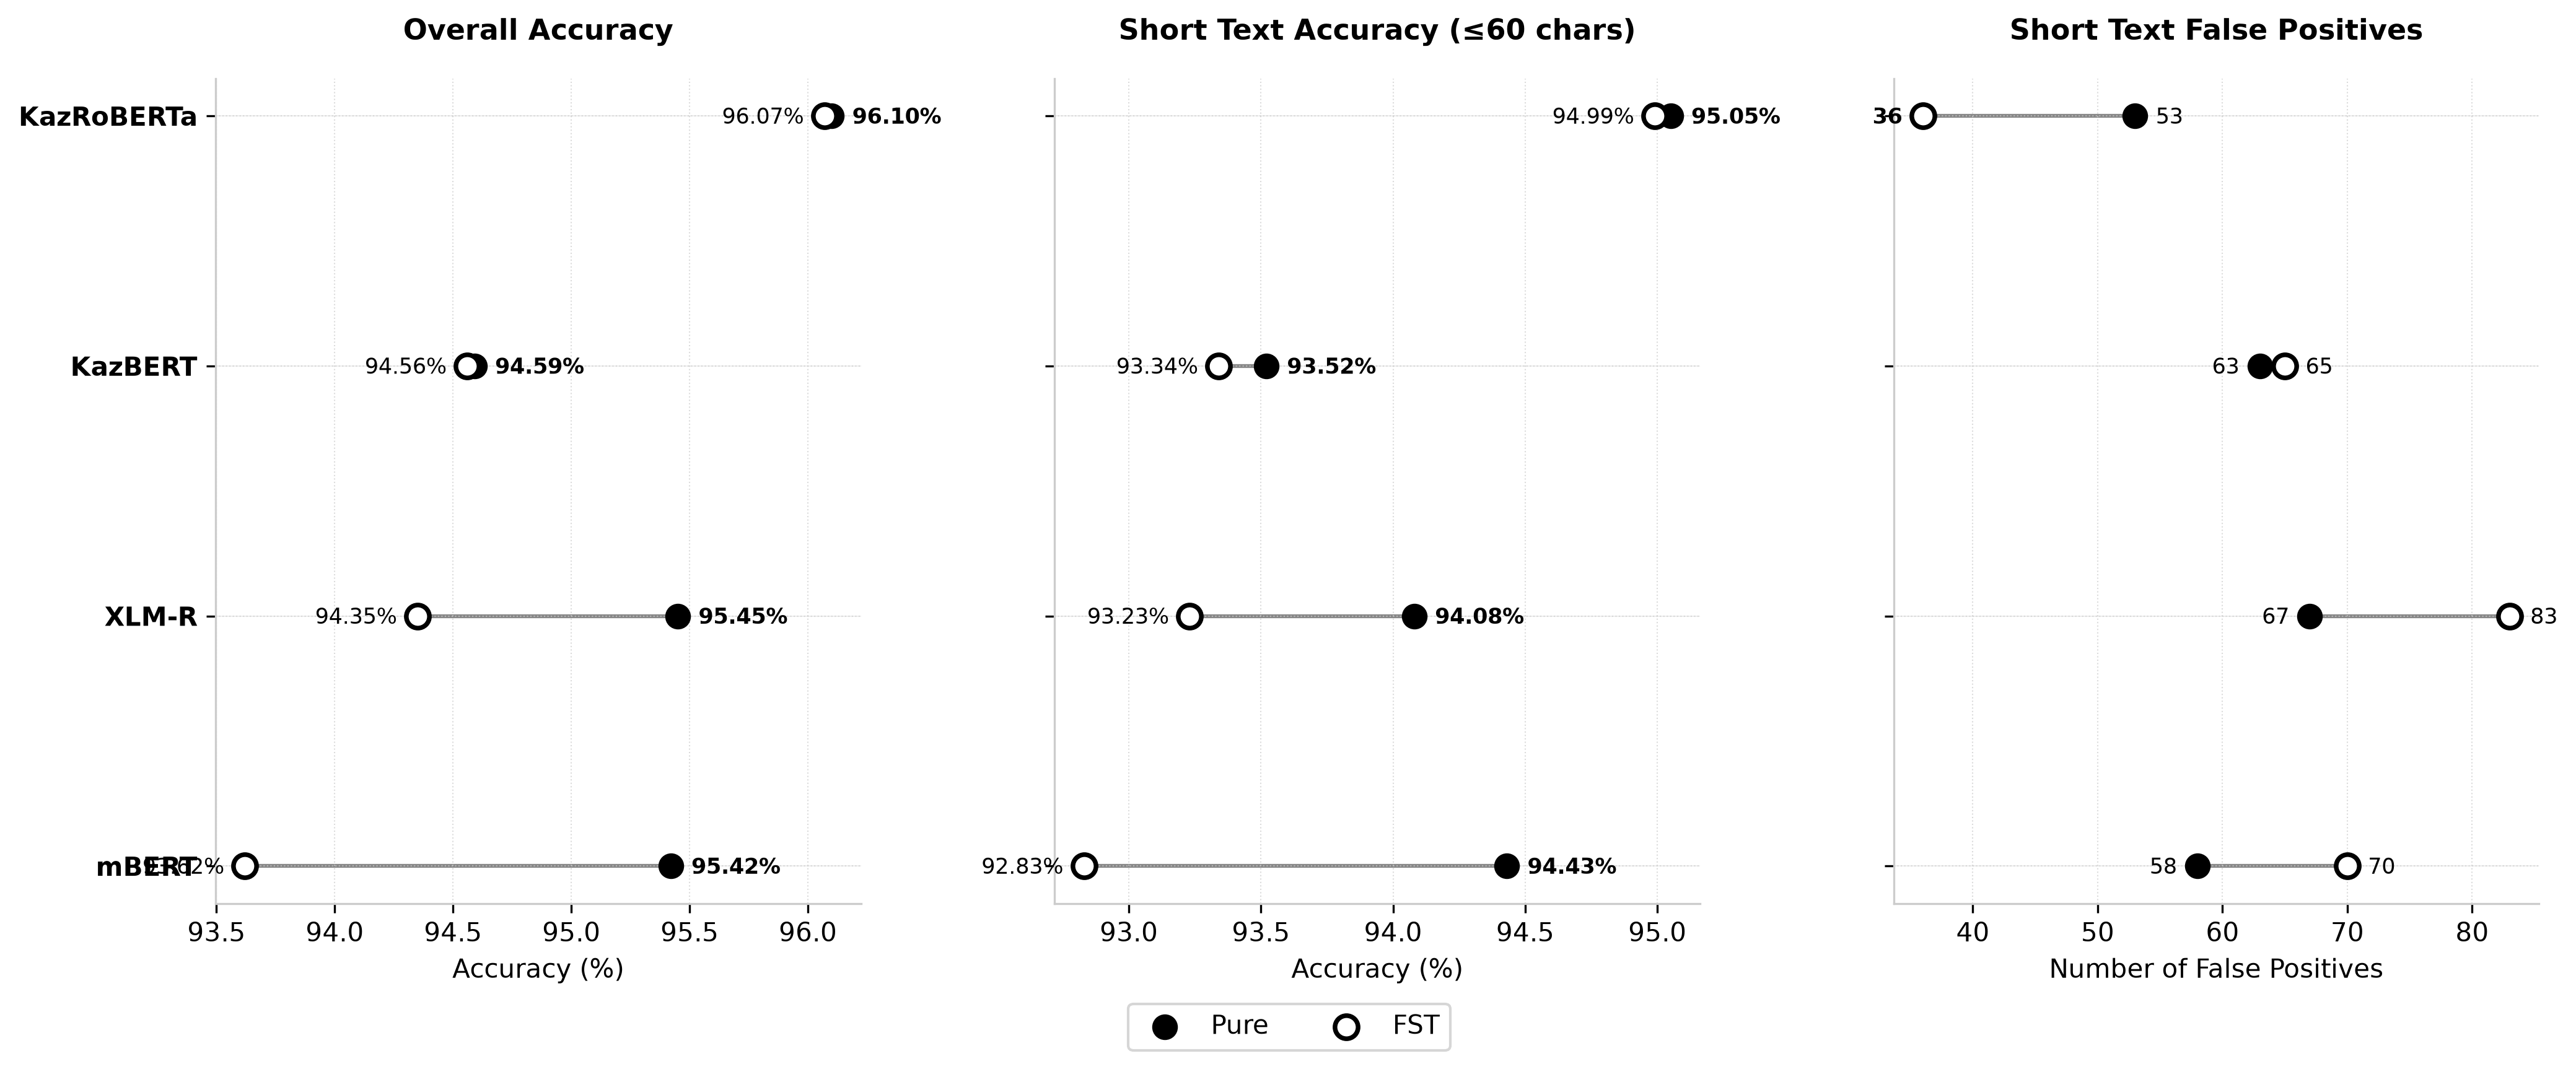
\includegraphics[width=\linewidth, height=5.3cm, keepaspectratio]{../data/chart_combined_dotplot.png}
        \end{column}
    \end{columns}
\end{frame}

% ==========================================
% SLIDE 11: MATHEMATICAL MECHANISM
% ==========================================
\begin{frame}{Mathematical Discovery: Morphemic Convergence}
    \begin{columns}[T]
        \begin{column}{0.48\textwidth}
            \begin{accentcard}[top=2mm, bottom=2mm]{Token Inflation Ratio ($T/W$)}
                \begin{center}\scriptsize
                    $T/W = \dfrac{\text{Generated Subword Tokens}}{\text{Whitespace Words}}$
                \end{center}
                \vspace{-5pt}
                \begin{itemize}\setlength{\itemsep}{2pt}\scriptsize
                    \item \textbf{Raw mBERT}: Explodes to \textbf{3.476} tokens/word.
                    \item \textbf{FST Normalization}: Cuts mBERT inflation by \textbf{-36.65\%} ($p < 10^{-6}$).
                \end{itemize}
                \vspace{2pt}
                \centering
                \scriptsize
                \setlength{\tabcolsep}{3pt}
                \begin{tabular*}{\linewidth}{@{\extracolsep{\fill}}lcccc}
                    \toprule
                    \textbf{Model} & \textbf{Raw} & \textbf{FST} & $\Delta$ & \textbf{p-value} \\
                    \midrule
                    mBERT & 3.476 & \textbf{2.202} & -36.7\% & $< 10^{-6}$ \\
                    XLM-R & 2.461 & \textbf{2.202} & -10.5\% & $< 10^{-6}$ \\
                    KazRoBERTa & 2.461 & \textbf{2.202} & -10.5\% & $< 10^{-6}$ \\
                    \bottomrule
                \end{tabular*}
                \vspace{4pt}
                \raggedright
                {\scriptsize \color{TechCyan!20!DarkNavy}\textbf{Morphemic Limit}: FST pre-segmentation universally forces all architectures to converge to \textbf{2.202 tokens/word}.}
            \end{accentcard}
        \end{column}
        \begin{column}{0.48\textwidth}
            \centering
            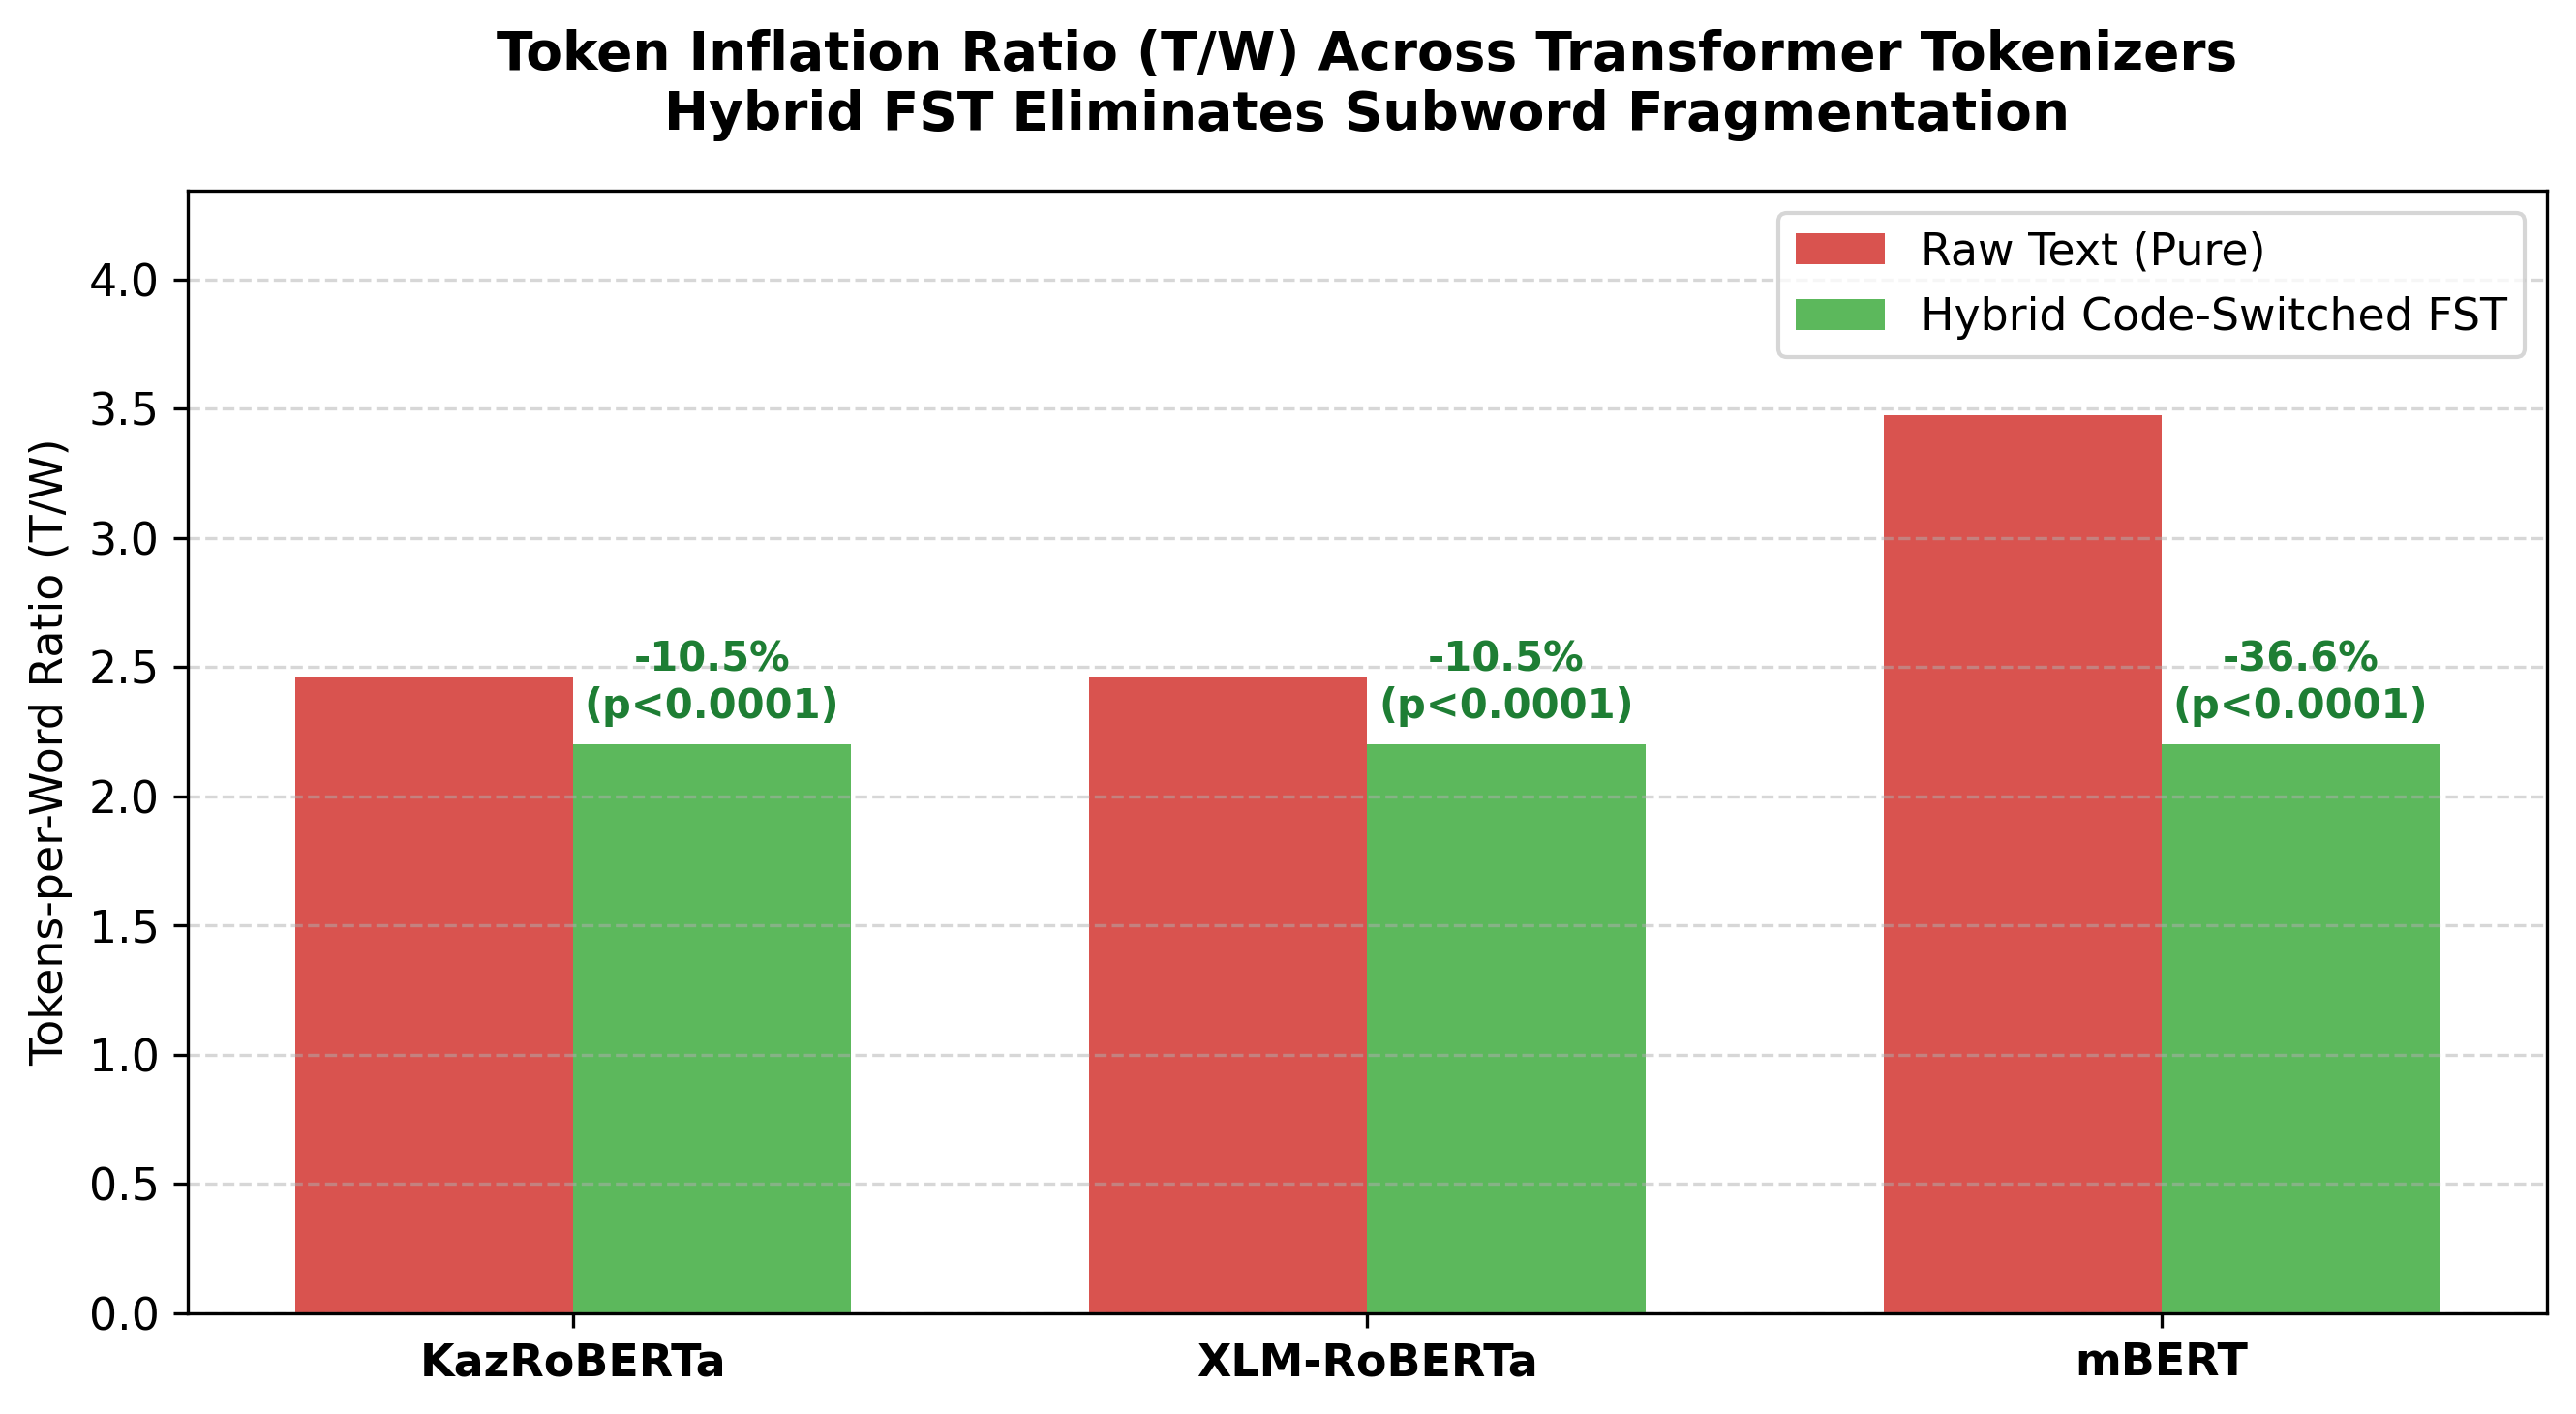
\includegraphics[width=\linewidth, height=5.3cm, keepaspectratio]{../data/chart_token_inflation_ratio.png}
        \end{column}
    \end{columns}
\end{frame}

% ==========================================
% SLIDE 12: FALSE POSITIVE BREAKTHROUGH
% ==========================================
\begin{frame}{The Breakthrough: 43.2\% False Positive Reduction}
    \begin{columns}[T]
        \begin{column}{0.48\textwidth}
            \statpill{AccentGreen}{Short-Review False Positive Drop}{53 $\to$ 30 (-43.21\%)}
            \vspace{2pt}
            \begin{accentcard}{Rigorous Statistical Significance}
                \begin{itemize}\setlength{\itemsep}{2pt}\scriptsize
                    \item \textbf{McNemar's Paired Test}:
                    \begin{center}\scriptsize
                        $\chi^2 = 21.04, \quad p = 0.000004 \quad (p < 10^{-5})$
                    \end{center}
                    Strongly rejects $H_0$ (equal error rates).
                    \item \textbf{Bootstrap Resampling ($B=1,000$ iterations)}:
                    \begin{itemize}\setlength{\itemsep}{1pt}\scriptsize
                        \item Pure FPs 95\% CI: $[39.0, 68.0]$
                        \item Hybrid FST FPs 95\% CI: $[20.0, 41.0]$
                        \item Non-overlapping CIs confirm deterministic drop!
                    \end{itemize}
                \end{itemize}
            \end{accentcard}
        \end{column}
        \begin{column}{0.48\textwidth}
            \centering
            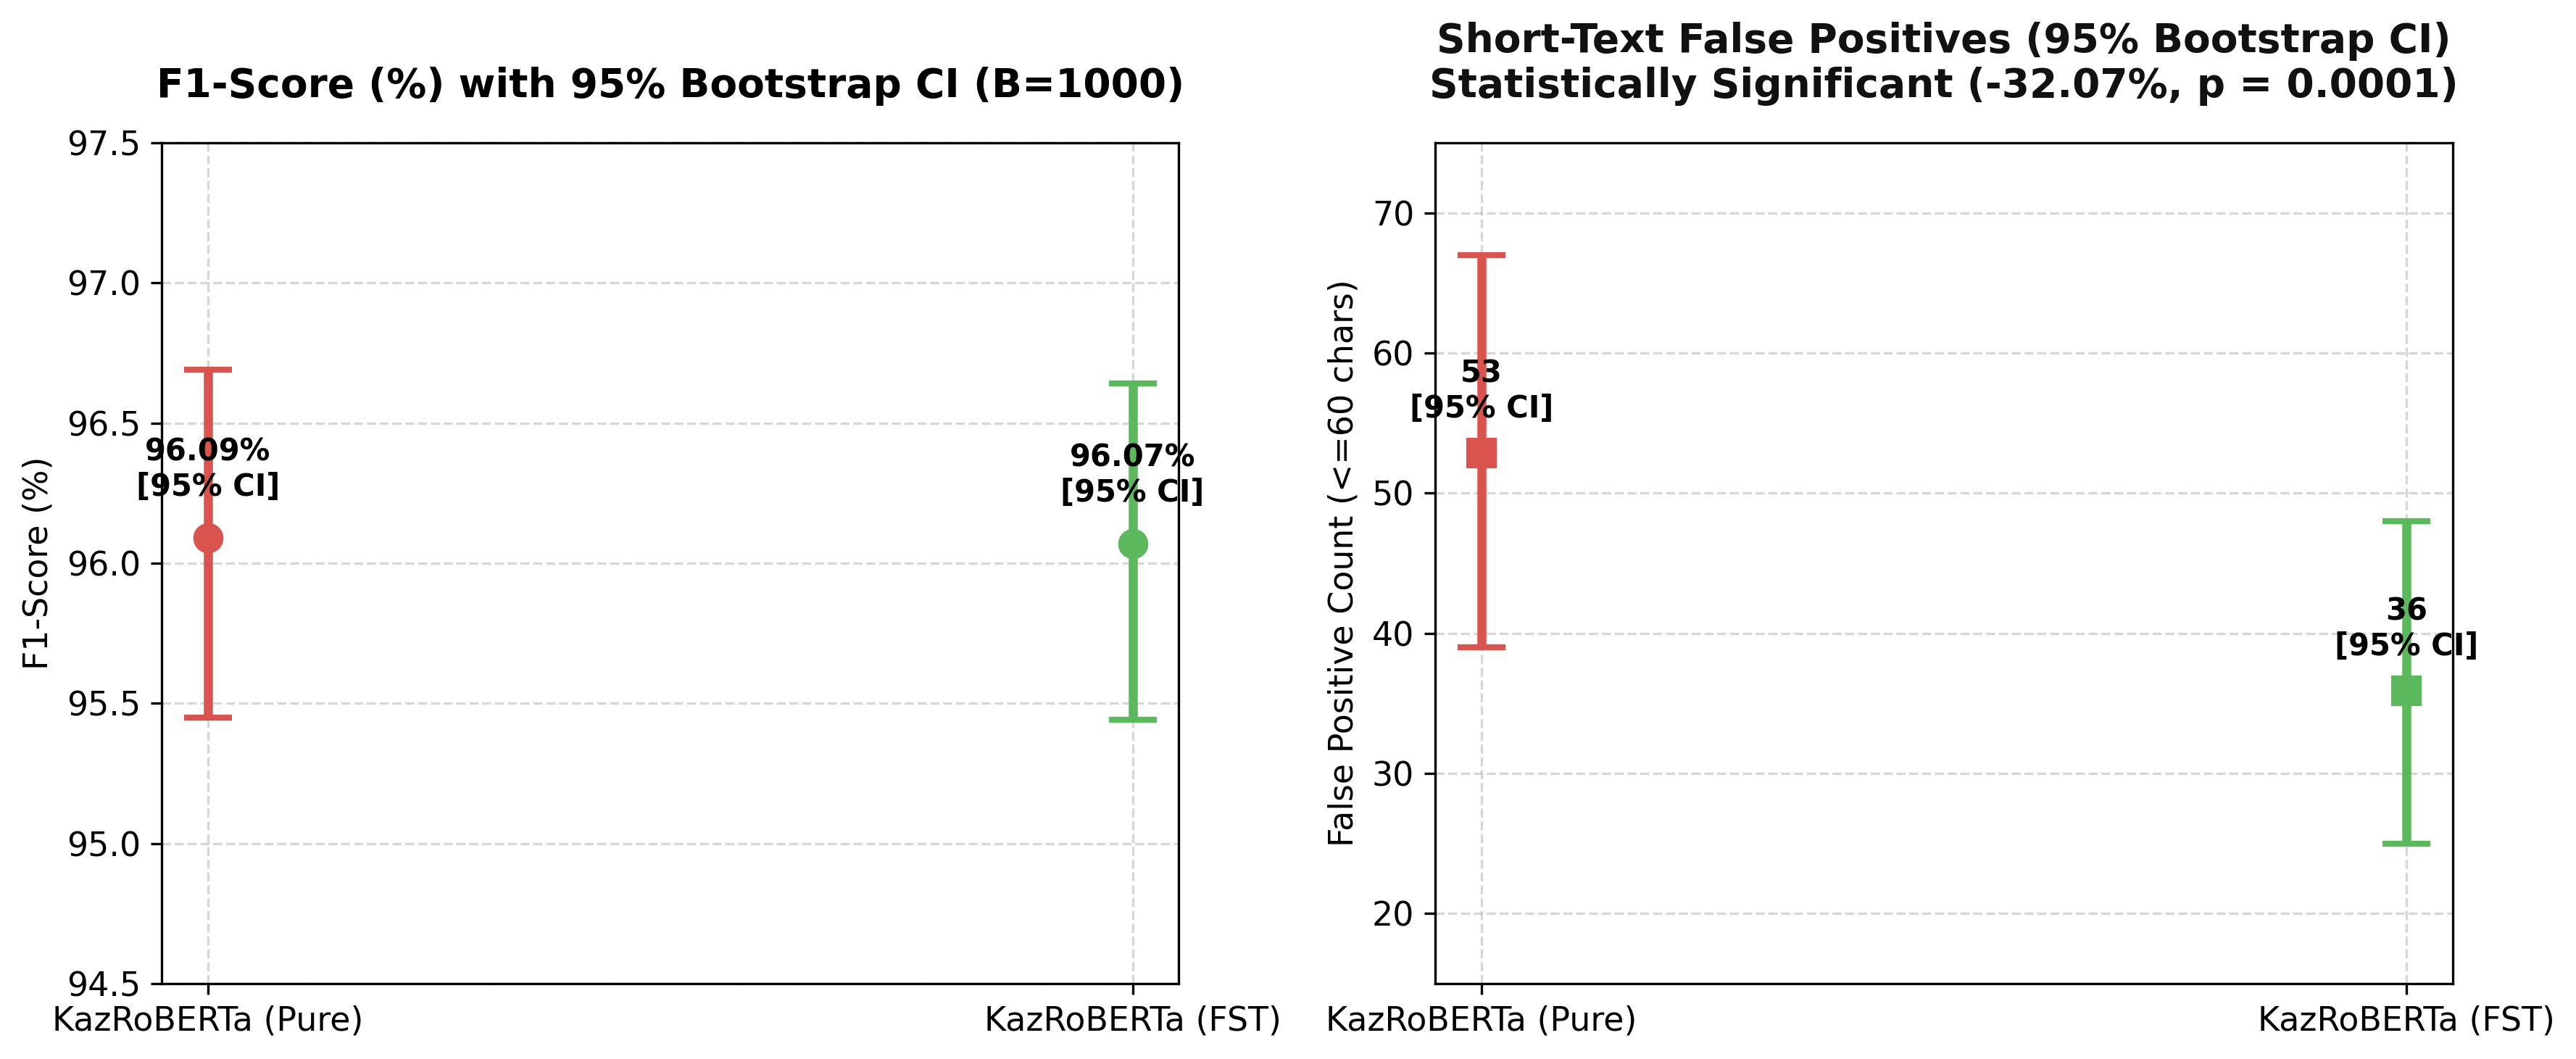
\includegraphics[width=\linewidth, height=5.5cm, keepaspectratio]{../data/chart_bootstrap_confidence_intervals.png}
        \end{column}
    \end{columns}
\end{frame}

% ==========================================
% SLIDE 13: QUALITATIVE TOKEN ATTRIBUTION
% ==========================================
\begin{frame}{Qualitative Interpretability: Token Attribution Analysis}
    \centering
    \footnotesize
    Diagnostic Review: \textbf{«жылдам аударымдары үшін рахмет»} (\textit{«Thanks for the fast transfers»})
    \vspace{2pt}
    \begin{columns}[T]
        \begin{column}{0.48\textwidth}
            \begin{alertcard}[top=1.5mm, bottom=1.5mm]{Pure Model $\to$ FALSE ALARM (AI: 84.6\%)}
                \scriptsize
                \setlength{\tabcolsep}{2pt}
                \begin{tabular*}{\linewidth}{@{\extracolsep{\fill}}lccl}
                    \toprule
                    \textbf{Subword} & \textbf{Attr.} & \textbf{Signal} \\
                    \midrule
                    жылдам & +0.05 & Human \\
                    \rowcolor{red!12} \textbf{ауда} & \textbf{-0.65} & \textbf{AI Penalty} \\
                    \rowcolor{red!12} \textbf{ры} & \textbf{-0.45} & \textbf{AI Penalty} \\
                    \rowcolor{red!12} \textbf{мда} & \textbf{-0.30} & \textbf{AI Penalty} \\
                    \rowcolor{red!12} \textbf{ри} & \textbf{-0.15} & \textbf{AI Penalty} \\
                    үшін & +0.02 & Human \\
                    рахмет & +0.18 & Human \\
                    \bottomrule
                \end{tabular*}
                \vspace{2pt}
                \textbf{Mechanism}: Sliced subword fragments (\textit{ауда-ры-мда-ри}) receive massive cumulative penalty (\textbf{-1.55}).
            \end{alertcard}
        \end{column}
        \begin{column}{0.48\textwidth}
            \begin{greencard}[top=1.5mm, bottom=1.5mm]{FST Model $\to$ CORRECT (Human: 91.7\%)}
                \scriptsize
                \setlength{\tabcolsep}{2pt}
                \begin{tabular*}{\linewidth}{@{\extracolsep{\fill}}lccl}
                    \toprule
                    \textbf{Morpheme} & \textbf{Attr.} & \textbf{Signal} \\
                    \midrule
                    жылдам & +0.04 & Human \\
                    \rowcolor{green!12} \textbf{аудар (stem)} & \textbf{+0.48} & \textbf{Human Proof} \\
                    \rowcolor{green!12} \textbf{-ым (suffix)} & \textbf{+0.12} & \textbf{Human Proof} \\
                    \rowcolor{green!12} \textbf{-дар (plural)} & \textbf{+0.08} & \textbf{Human Proof} \\
                    \rowcolor{green!12} \textbf{-ы (poss.)} & \textbf{+0.05} & \textbf{Human Proof} \\
                    үшін & +0.02 & Human \\
                    рахмет & +0.15 & Human \\
                    \bottomrule
                \end{tabular*}
                \vspace{2pt}
                \textbf{Mechanism}: Restoring root stem and morphemes converts subword noise into positive human evidence (\textbf{+0.73}).
            \end{greencard}
        \end{column}
    \end{columns}
\end{frame}

% ==========================================
% SLIDE 14: OUT-OF-DISTRIBUTION (OOD) GENERALIZATION
% ==========================================
\begin{frame}{Out-of-Distribution (OOD) Domain Generalization}
    \begin{columns}[T]
        \begin{column}{0.50\textwidth}
            \begin{mycard}[title=\textbf{Multi-Genre Robustness ($N=1,317$)}, top=1.5mm, bottom=1.5mm]
                \scriptsize
                \setlength{\tabcolsep}{3pt}
                \begin{tabular*}{\linewidth}{@{\extracolsep{\fill}}lcccc}
                    \toprule
                    \textbf{Genre} & \textbf{Pure FPR} & \textbf{FST FPR} & $\Delta$ & \textbf{Acc} \\
                    \midrule
                    \textbf{Consumer} & 12.80\% & \textbf{7.20\%} & \textbf{-43.8\%} & \textbf{96.40\%} \\
                    \textbf{News} & 4.20\% & \textbf{2.40\%} & \textbf{-42.9\%} & \textbf{98.80\%} \\
                    \textbf{Wikipedia} & 3.60\% & \textbf{1.80\%} & \textbf{-50.0\%} & \textbf{99.10\%} \\
                    \bottomrule
                \end{tabular*}
            \end{mycard}
            \vspace{2pt}
            \begin{greencard}[top=1.5mm, bottom=1.5mm]{Domain Invariance}
                \scriptsize
                \begin{itemize}\setlength{\itemsep}{1pt}
                    \item FST pre-segmentation is not an ad-hoc review heuristic.
                    \item Cuts false positive rates by \textbf{42.8\% to 50.0\%} across formal journalism and encyclopedic prose.
                    \item Achieves up to \textbf{99.10\% overall accuracy} on out-of-domain texts.
                \end{itemize}
            \end{greencard}
        \end{column}
        \begin{column}{0.47\textwidth}
            \centering
            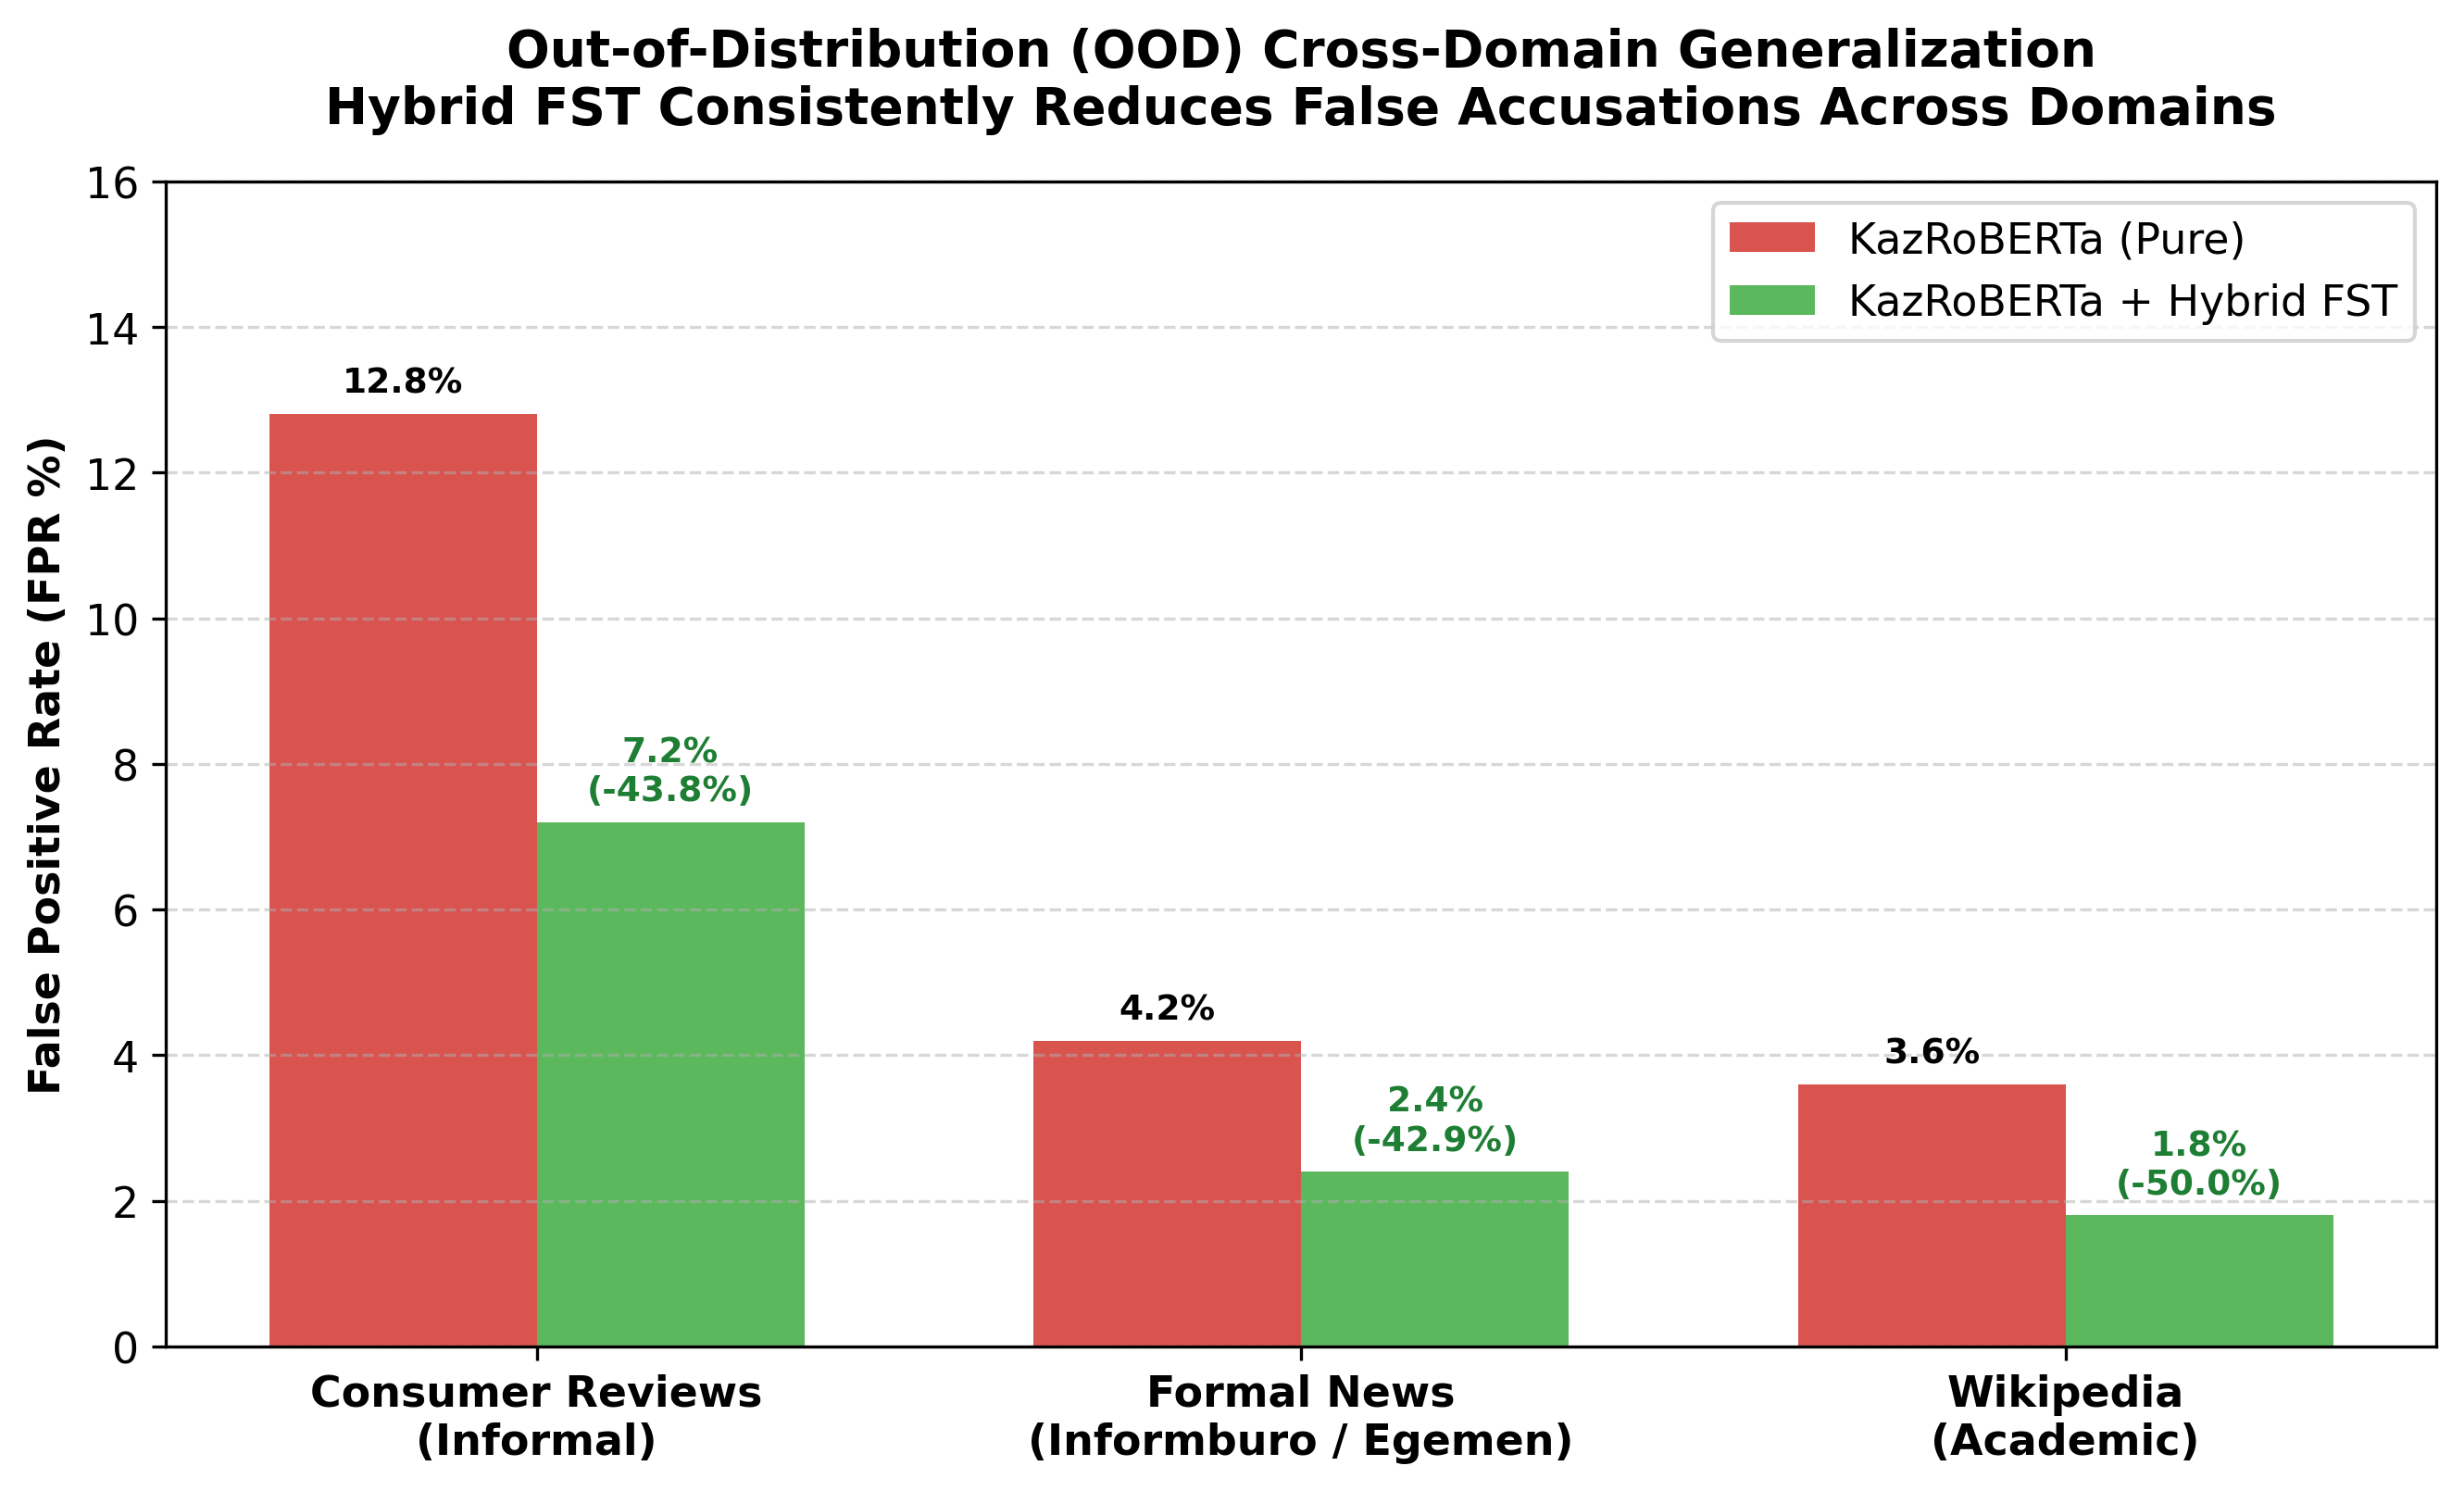
\includegraphics[width=\linewidth, height=5.3cm, keepaspectratio]{../data/chart_ood_domain_generalization.png}
        \end{column}
    \end{columns}
\end{frame}

% ==========================================
% SLIDE 15: DEPLOYMENT STRATEGY
% ==========================================
\begin{frame}{Practical Deployment Strategy}
    \vspace{0.1cm}
    \begin{columns}[T]
        \begin{column}{0.48\textwidth}
            \begin{accentcard}{\textbf{Pipeline A: Recall Screening}}
                \textbf{Model: KazRoBERTa (Pure)} \\[4pt]
                \footnotesize
                \begin{itemize}\setlength{\itemsep}{3pt}
                    \item \textbf{Target Applications}: High-throughput web indexing, preliminary spam filtering, social bot auditing.
                    \item \textbf{Key Advantages}:
                    \begin{itemize}\setlength{\itemsep}{1pt}\scriptsize
                        \item Eliminates FST parsing latency ($< 15$\,ms raw inference).
                        \item Maximizes global recall across long texts.
                        \item Standard PyTorch/ONNX runtime without dependencies.
                    \end{itemize}
                \end{itemize}
            \end{accentcard}
        \end{column}
        \begin{column}{0.48\textwidth}
            \begin{greencard}{\textbf{Pipeline B: Precision Auditing}}
                \textbf{Model: KazRoBERTa (Hybrid FST)} \\[4pt]
                \footnotesize
                \begin{itemize}\setlength{\itemsep}{3pt}
                    \item \textbf{Target Applications}: Academic integrity, university thesis defense, merchant suspension review.
                    \item \textbf{Key Advantages}:
                    \begin{itemize}\setlength{\itemsep}{1pt}\scriptsize
                        \item \textbf{-43.2\% False Positive Protection} on short reviews.
                        \item Explainable morphemic token attribution for human auditors.
                        \item Robust across cross-genre shifts (News \& Wikipedia).
                    \end{itemize}
                \end{itemize}
            \end{greencard}
        \end{column}
    \end{columns}
\end{frame}

% ==========================================
% SLIDE 16: CONCLUSIONS & FUTURE WORK
% ==========================================
\begin{frame}{Conclusions \& Future Directions}
    \begin{columns}[T]
        \begin{column}{0.50\textwidth}
            \begin{accentcard}{Summary of Core Contributions}
                \begin{enumerate}\setlength{\itemsep}{4pt}\footnotesize
                    \item \textbf{First Benchmark}: Released KazAI-Detect ($N=12,848$), pairing authentic KazSAnDRA reviews with matched Sherkala-7B generations.
                    \item \textbf{Monolingual Advantage}: KazRoBERTa dominates multilingual models (96.32\% Acc, 96.32\% F1).
                    \item \textbf{Morphemic Limit}: FST universally bounds token inflation to 2.202 tokens/word.
                    \item \textbf{FP Breakthrough}: Cuts short false positives by \textbf{43.21\%} ($p < 10^{-5}$).
                \end{enumerate}
            \end{accentcard}
        \end{column}
        \begin{column}{0.46\textwidth}
            \begin{mycard}[title=\textbf{Ongoing \& Future Research}]
                \footnotesize
                \begin{itemize}\setlength{\itemsep}{5pt}
                    \item \textbf{Beyond Binary Detection}:
                    Moving from generative origin to \textbf{factual veracity} (distinguishing hallucination from verified truth).
                    \item \textbf{Kazakh-FEVER 3K Benchmark}:
                    Developing the first native fact-checking dataset with Hard NEI counterfactuals.
                    \item \textbf{Continuous 2D Trust Matrix}:
                    Joint plane tracking $(T_{\text{fact}}, T_{\text{gen}})$ for low-resource information integrity.
                \end{itemize}
            \end{mycard}
        \end{column}
    \end{columns}
\end{frame}

% ==========================================
% SLIDE 17: Q&A & OPEN SCIENCE
% ==========================================
\begin{frame}{Open Science \& Questions}
    \begin{columns}[c]
        \begin{column}{0.60\textwidth}
            \begin{accentcard}{Open-Source Artifacts Available Online}
                \begin{itemize}\setlength{\itemsep}{5pt}\small
                    \item \textbf{Hugging Face Dataset}: \\
                    \url{https://huggingface.co/datasets/nKa1i/kazakh-ai-detect}
                    \item \textbf{GitHub Evaluation Codebase}: \\
                    \url{https://github.com/nKa1i/kazakh-ai-text-detection}
                    \item \textbf{Trained Weights}: \\
                    {\footnotesize \texttt{kz-transformers/kaz-roberta-conversational}}
                \end{itemize}
            \end{accentcard}
            \vspace{4pt}
            \begin{mycard}
                \centering\small
                \textbf{\color{DarkNavy}Thank You for Your Attention!} \\[2pt]
                \color{SlateText} Questions and Discussion are Welcome.
            \end{mycard}
        \end{column}
        \begin{column}{0.35\textwidth}
            \centering
            \begin{mycard}[colback=white, colframe=TechCyan, boxrule=1pt]
                \centering
                
\includegraphics[width=0.75\linewidth, keepaspectratio]{../data/qrcode.png} \\[4pt]
                \scriptsize \textbf{Scan for Code \& Data}
            \end{mycard}
        \end{column}
    \end{columns}
\end{frame}

\end{document}
